\section{Farbe}

\subsection{Was ist Farbe?}

\begin{itemize}
    \item \textbf{Physikalisch}, Lichtzusammensetzung, Elektromagnetischestrahlen
    \item \textbf{Physologisch}, Warnehmung und Interpretation
\end{itemize}

\textit{Farbe besteht aus:}

\begin{itemize}
    \item Farbton/Farbe
    \item Farbstich/Sättigung
    \item Helligkeit
\end{itemize}

\subsection{Farbe eines Objektes}

\textit{
    Ein Objekt nimmt Farbe auf und strahlt Farbe ab.
    Die Farbe des Objektes ist definiert durch die abgestrahlte
    Farbe.
}

\begin{itemize}
    \item Beleuchtung (Illumination)
    \item Reflektion (Reflection)
    \item Farbsignal (Color Signal)
\end{itemize}

\subsection{Licht besteht aus?}

\textit{
    Licht besitzt verschiedene Wellenlängen,
    Kombinationen dieser Frequenzen ergeben eine Farbe.
}

\begin{itemize}
    \item Sichtbares Licht (380mn - 780mn)
    \item Infrarot (780mn+)
    \item Ultraviolet (-380mn)
\end{itemize}

\textit{1nm = 10\AA (\AA ngström)} \\
\textit{1\AA = \o Atom}

\subsection{Das Auge}

\textit{
    Das Auge besteht aus; \textbf{Iris} (Kreisring mit radialen Muskel und Lichteinschränken),
    \textbf{Linse} (Fokussieren), \textbf{Pupille} (Öffnung, durch Iris kontrolliert), \textbf{Photorezeptoren} (Nehmen das Licht wahr) und \textbf{Retina}
    (Farb- und Lichtaufnahme am Rand des Auges)
} \\
\\
\textit{
    Die Retina besteht aus 75-100 $10^6$ Stäbchen/rods (Lichtintensität) und
    6-7 $10^6$ Zäpfchen/cones (Farbe). Die Forea ist der dichteste Platz.
}

\subsection{Wie sehen wir Farbe?}

\textit{Durch die 3 Arten von Zäpfchen:}

\begin{tabular}{ccccc}
    Kurz (S) & & Mittel (M) & & Lang (L) \\
    Blau     & & Grün       & & Rot \\
    440mn    & & 530mn      & & 560mn \\
    1        &:& 5          &:& 10 \\
\end{tabular}

\textit{
	Weiss ist eine Kombination von Wellenlängen. Es gibt verschiedene Verteilung für Weiss.
}

\subsection{Wahrnehmung}

\textit{Grün 530mn wird am intensivsten wargenommen}

\textit{
    Die Helligkeitswahrnehmung zwischen Stäbchen und
    Zäpfchen ist unterschiedlich
}

\subsection{Farbsysteme}

\textit{
	Nicht alle existierenden Farben (CIE) sind mit allen System darstellbar!
}

\begin{itemize}
    \item \textbf{RGB} (Monitor, Spotligths,Pointilismus), \\
          additiv, C = (Rot, Grün, Blau)
          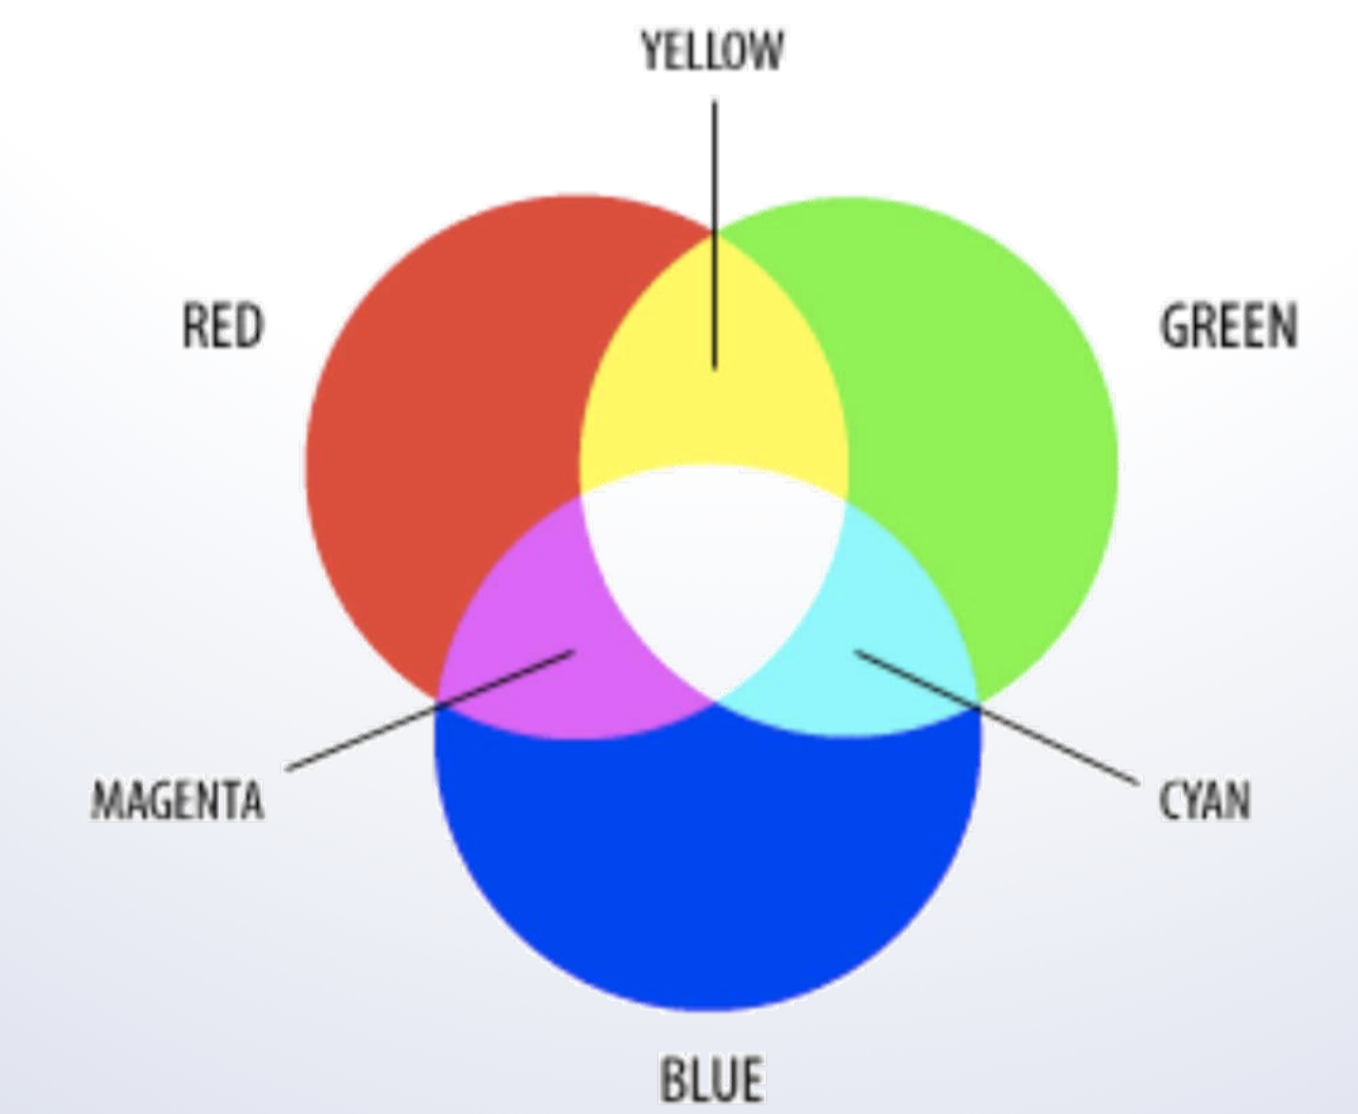
\includegraphics[width=0.3\textwidth]{assets/rgb_additiv.png}
          
    \item \textbf{CMY} (Drucken), \\
          subtraktiv, C = (Cyan, Magenta, Yellow) \\
          Komplementärfarbe von RGB \\
          $(C,M,Y) = (1,1,1) - (R,G,B)$
          
    \item \textbf{CMYK}, CMY Mit Schwarz erweitert, \\
          K = min(Cyan, Magenta, Yellow) \\
          $C = C - K$, $M = M - K$, $Y = Y - K$
          
    \item \textbf{HSV}, \
          Farbton (Hue) / \
          Reinheit,Sättigung (Saturation) / \
          Intensität (Value)
          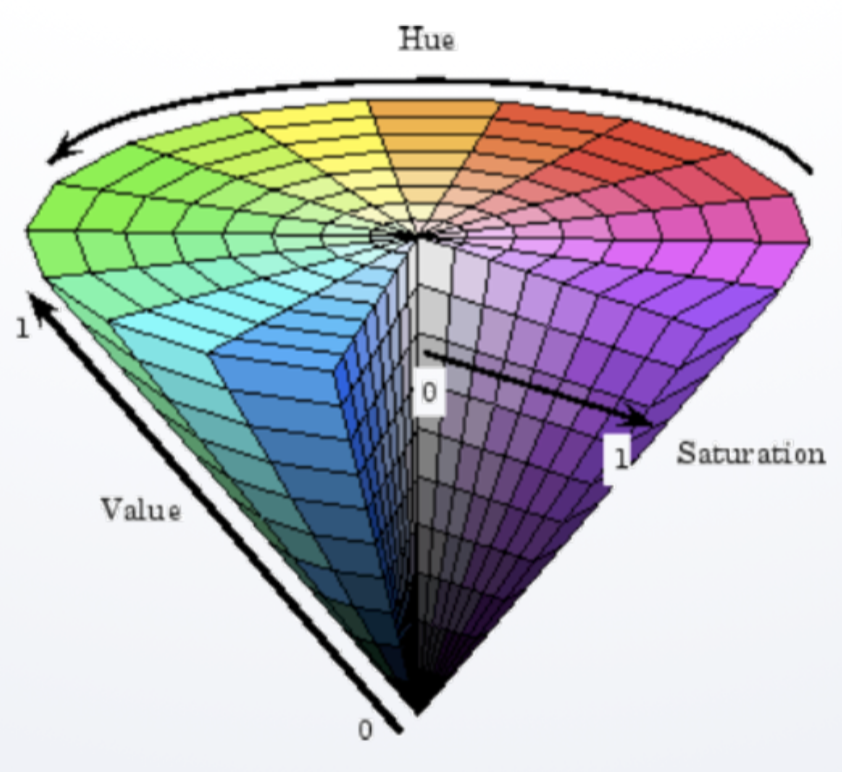
\includegraphics[width=0.3\textwidth]{assets/hsv_farbsystem.png}
          
    \item \textbf{YUV} (Alte Fernseher, Y= Helligkeit, UV = 1/4 Auflösung Farbkorrektur)\\
          Y = $0.229*R+0.587G+0.114*B$, \\
          U = $0.436(B-Y)/(1-0.114)$, \\
          V = $0.615(R-Y)/(1-0.299)$
          
    \item \textbf{CIE-Lab}, absolutes Farbsystem \\
          Achsensystem mit Helligkeit (L) als Y-Achse und X/Z-Achse definieren Farbunterschiede \\
          a: rot – grün Achse \\
          b: gelb – blau Achse
\end{itemize}

\subsection{Additives Farbsystem}

\textit{Farben additeren} \\
\textit{(1,1,1) = Weiss, (0,0,0) = Schwarz}

\subsection{Subtraktives Farbsystem}

\textit{Farben absorbieren / filtern} \\ 
\textit{(0,0,0) = Weiss, (1,1,1) = Schwarz}

\subsection{Farben Konvertieren}

\textit{Zu Grau: $I = 0.229*R+0.587G+0.114*B$} \\

\textit{RGB <> CMY: }x
$\begin{pmatrix} C \\ M \\ Y \end{pmatrix} =
\begin{pmatrix} 1 \\ 1 \\ 1 \end{pmatrix} -
\begin{pmatrix} R \\ G \\ B \end{pmatrix}$ \\

\subsubsection{RGB -> CMYK}
\textit{devide by 255 to get range from 0-1}\\
$R' = R / 255$\\
$G' = G / 255$\\
$B' = B / 255$\\
\\
$K = 1-max(R',G'.B')$\\
$C = (1-R'-K) / (1-K)$\\
$M = (1-G'-K) / (1-K)$\\
$Y = (1-B'-K) / (1-K)$\\

\subsubsection{CMYK -> RGB}

$R = 255 \cdot (1-C) \cdot (1-K)$\\
$G = 255 \cdot (1-M) \cdot (1-K)$\\
$B = 255 \cdot (1-Y) \cdot (1-K)$\\

\subsubsection{RGB -> HSV}
\textit{devide by 255 to get range from 0-1}\\
$R' = R / 255$\\
$G' = G / 255$\\
$B' = B / 255$\\

$Cmax = max(R',G',B')$\\
$Cmin = min(R',G',B')$\\
$\Delta = Cmax - Cmin$\\

\textbf{Hue calculation}\\

$H = \begin{cases}
	0^\circ     & \text{ falls } \Delta = 0 \\
	60^\circ \cdot (\frac{G'-B'}{\Delta}mod 6) & \text{ falls } Cmax = R' \\
	60^\circ \cdot (\frac{B'-R'}{\Delta}+2) & \text{ falls } Cmax = G' \\
	60^\circ \cdot (\frac{R'-G'}{\Delta}+4) & \text{ falls } Cmax = B' \\
\end{cases}$

\textbf{Saturation calculation}\\

$S = \begin{cases}
	0     & \text{ falls } Cmax = 0 \\
	\frac{\Delta}{Cmax} & Cmax \neq 0 \\
\end{cases}$

\textbf{Value calculation}\\
$V = Cmax$

\subsubsection{HSV -> RGB}

\textit{$0 \leq H \leq 360, 0 \leq S \leq 1, 0 \leq V \leq 1$}

$C = V \cdot S$\\
$X = C \cdot (1 - |(H / 60^\circ) mod 2-1|)$\\
$m = V - C$\\

$(R',G',B') = \begin{cases}
	(C,X,0)	& \text{ falls } 0^\circ \leq H \leq 60^\circ \\
	(X,C,0)	& \text{ falls } 60^\circ \leq H \leq 120^\circ \\
	(0,C,X)	& \text{ falls } 120^\circ \leq H \leq 180^\circ \\
	(0,X,C)	& \text{ falls } 180^\circ \leq H \leq 240^\circ \\
	(X,0,C)	& \text{ falls } 140^\circ \leq H \leq 300^\circ \\
	(C,0,X)	& \text{ falls } 300^\circ \leq H \leq 360^\circ \\
\end{cases}$

$(R,G,B) = ((R'+m)\cdot255, (G'+m)\cdot255, (B'+m)\cdot255)$

\textit{HSV <> RGB: }\\
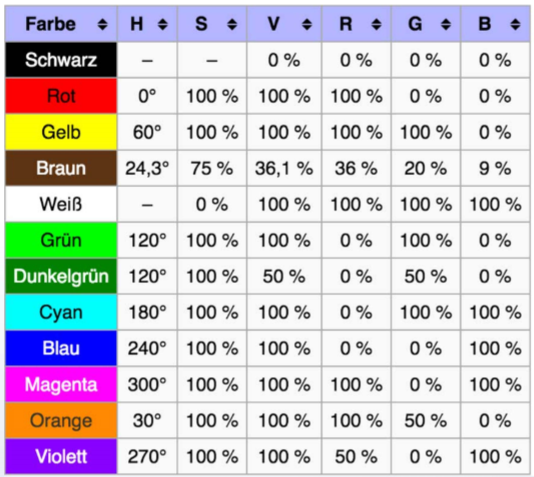
\includegraphics[width=0.4\textwidth]{assets/hsv-rgb.png}
\\
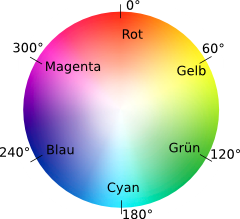
\includegraphics[width=0.25\textwidth]{assets/hsv_hue.png}

\subsection{Gamma Korrektur}

\textit{
    Erreichen von gleichmässiger Verteilung der Helligkeit / Kontrast.
    Das Empfinden der Helligkeit ist nicht linear.
} \\
\\
\textit{
    Korrektur der Helligkeit des Bildes mit Gamme Wert. Wichtig für Bildschirme einstellen.
    Beim einstellen der Monitore Grauwerte mit echten Werten vergleichen (Gamma Test Pattern).
    50\% schwarz und 50\% weiss einer Fläche (z.B. Punkte) sollte gleich sein wie 50\% grau
}

\subsection{Normfarbtafel / CIE Farbsystem}
\begin{itemize}
	\item kann alle Farben darstellen
	\item Spektralfarben = Farbe am Rand mit Wellenlänge
	\item Farben zwischen zweie Farben mischbar
	\item Komplementärfarben gehen durch Weiss
	\item Achtung: Keine Spektralfarbe am Rande zwischen UV und Infrarot
\end{itemize}

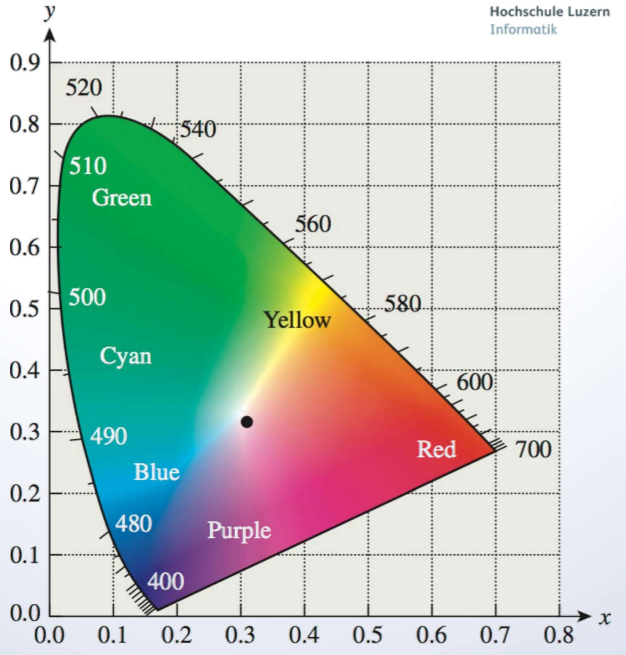
\includegraphics[width=0.4\textwidth]{assets/color-cie.png}

\subsection{Helligkeitswahrnehmung}

\textit{Helligkeit wird logarithmisch wahrgenommen, Webers Law}

$\frac{\Delta I}{I} = C$ \\
$\log (I + \Delta I) - \log(I) = Const$

\textit{Helligkeitsunterschied im dunkeln nehmen wir stärker wahr}
 
\subsection{Nibs (Lichtdichte)}

\textit{
    Gibt Helligkeitsdichte für Auge an. 10nits werden stärker wargenommen denn 100nits.
    Heisst, weniger Licht wird stärker wargenommen.
}

\subsection{Mach bending}

\textit{
    Optische Illusion, bei zwei verschiedenen Grauwerten nebeneinander
    unterschieden sich diese vermeidlich stärker.
}

\subsection{Farbtäschung}

\textit{
    Farbe wird abhängig durch Umgebung anders wahrgenommen
    (Dunkler, Heller). Optische Illusionen
}

\subsection{HD,UHD,UK}

\textit{Unterscheiden sich durch Pixelauflösung.}

\subsection{Was ist HDR?}

\textit{
    \textbf{High Dynamic Range}, speichert zusätzlichen Wert um
    Helligkeitsunterschiede besser unterschieden zu können
    (RGB-Pixelwerte propertianal zum Licht).
    Detailreichere dunkel und helle Spots, weniger Verlust
    durch Farben mit weniger Helligkeitsunterschiede.
}

\subsection{Begriffe}

\begin{tabular}{r|l}
    \textbf{Natürliches Licht}  & Gemisch aus verschiedenen \\
                                & Lichtwellen / Frequenzen \\
    \textbf{Spektralfarben}     & reine Farbfrequenz; Alle Farben \\
                                & am Rand des CIE-Farbsystems \\
    \textbf{Spektrum}           & Alle Frequenzen und deren \\
                                & Verteilung \\
    \textbf{Spektralverteilung} & Charakterisiert die Farbe, definiert \\
                                & durch Frequenzen \\
                                & (Bsp. Verschiedenes Weiss) \\
    \textbf{Komplementärfarben} & Addieren ergeben Grau, \\
                                & gegenüberligende Farben im \\
                                & CIE-Farbsystem durch Weiss
\end{tabular}
